\documentclass[12pt, a4paper]{report}
\usepackage{epsfig}
\usepackage{subfigure}
%\usepackage{amscd}
\usepackage{amssymb}
\usepackage{amsbsy}
\usepackage{amsmath}
\usepackage{amsthm}
\usepackage{framed}
\usepackage{subfiles}
%\usepackage[dvips]{graphicx}
\usepackage{natbib}
\bibliographystyle{chicago}
\usepackage{vmargin}
% left top textwidth textheight headheight
% headsep footheight footskip
\setmargins{3.0cm}{2.5cm}{15.5 cm}{22cm}{0.5cm}{0cm}{1cm}{1cm}
\renewcommand{\baselinestretch}{1.5}
\pagenumbering{arabic}
\theoremstyle{plain}
\newtheorem{theorem}{Theorem}[section]
\newtheorem{corollary}[theorem]{Corollary}
\newtheorem{ill}[theorem]{Example}
\newtheorem{lemma}[theorem]{Lemma}
\newtheorem{proposition}[theorem]{Proposition}
\newtheorem{conjecture}[theorem]{Conjecture}
\newtheorem{axiom}{Axiom}
\theoremstyle{definition}
\newtheorem{definition}{Definition}[section]
\newtheorem{notation}{Notation}
\theoremstyle{remark}
\newtheorem{remark}{Remark}[section]
\newtheorem{example}{Example}[section]
\renewcommand{\thenotation}{}
\renewcommand{\thetable}{\thesection.\arabic{table}}
\renewcommand{\thefigure}{\thesection.\arabic{figure}}
\title{Research notes: linear mixed effects models}
\author{ } \date{ }


\begin{document}
	\author{Kevin O'Brien}
	\title{Mixed Models for Method Comparison Studies}
	
	\addcontentsline{toc}{section}{Bibliography}
	
	
	
	
	%	
	%	\citet{schabenberger} describes the examination of model-data agreement as comprising several elements; \begin{itemize}
	%		\item residual analysis,
	%		\item goodness of fit,
	%		\item collinearity diagnostics
	%		\item influence analysis.
	%	\end{itemize}
	%	
	%\end{abstract}
	\chapter{Residual Analysis and Influence Diagnostics for Method Comparison}
	Model validation and model appraisal are vital parts of the modelling process, yet are too often overlooked. Using a small set of simple measures and methods, such as the AIC and $R^2$ measures, is insufficient to properly assess the usefulness of a fitted model. In classical linear models model diagnostics are now considered a required part of any statistical analysis, and the methods are commonly available in statistical packages and standard textbooks on applied regression. A full and comprehensive
	analysis that comprises residual analysis and influence analysis for testing model assumptions, should be carried out. However it has been noted by several papers \citep{Christensen, schabenberger} that model diagnostics do not often accompany LME model analyses. Furthermore, a suite of dagnostic procedures designed for method comparison should be adopted.


\section{Influence Diagnostics}
Model diagnostic techniques can determine whether or not the distributional assumptions are satisfied, but also to assess the influence of unusual observations. Following model specification and estimation, it is of interest to explore the model-data agreement by raising pertinent questions. \citet{pb} provide some insight into how to compute and interpret model diagnostic plots for LME models. Unfortunately this aspect of LME theory is not as expansive as the corresponding body of work for Linear Models. Their particular observations will be reverted to shortly. Further to the analysis of residuals, \citet{schabenberger} recommends the examination of the following questions:
	\begin{itemize}
		\item Does the model-data agreement support the model assumptions?
		\item Should model components be refined, and if so, which components? For example, should certain explanatory variables
		be added or removed, and is the covariance of the observations properly specified?
		\item Are the results sensitive to model and/or data? Are individual data points or groups of cases particularly
		influential on the analysis?
	\end{itemize}
	
	The last of these three questions, regarding influential points, is of particular interest in the context of Method Comparison. After fitting an LME model, it is important to carry put model diagnostics to check whether distributional assumptions for the residuals as satisfied and whether the fit the model is sensitive to unusual assumptions. The process of carrying out model
	diagnostic involves several informal and formal techniques, which will mentioned throughout the chapter.

Influential points have a large influence on the fit of the model. Influential points are a set of one or more observations whose removal would cause a different conclusion in the analysis, e.g. substantially changes the estimate of the regression coefficients. \citet{west} remarks that influence diagnostics play an important role in the interpretation of results, because influential data can negatively influence the statistical model and generalizability of the model. \citet{schabenberger} remarks that the concept of critiquing the model-data agreement applies in mixed models in the same way as in linear
	fixed-effects models. In fact, because of the more complex model structure, you can argue that model and
	data diagnostics are even more important \citep{west}.
	%Influential points have a large influence on the fit of the model. 
	
	%One approach for determining influential points is to compare the fit of the model with and without each observation.
	
	%The basic rationale behind identifying influential data is that when iteratively single units are omitted from the data, models based on these data should not produce substantially different estimates. 


\section{Model Diagnostics for Roy's Models}

Further to previous work, this section revisits case-deletion and residual diagnostics, and explores how approaches devised by  \citet{Galecki} can be used to appraise Roy's model. These authors specifically look at Cook's Distances and Likelihood Distances.
%	For the Roy Model, Cook's Distances may also be generated using the \textbf{\textit{predictmeans}}
%	





\begin{figure}[h!]
	\centering
	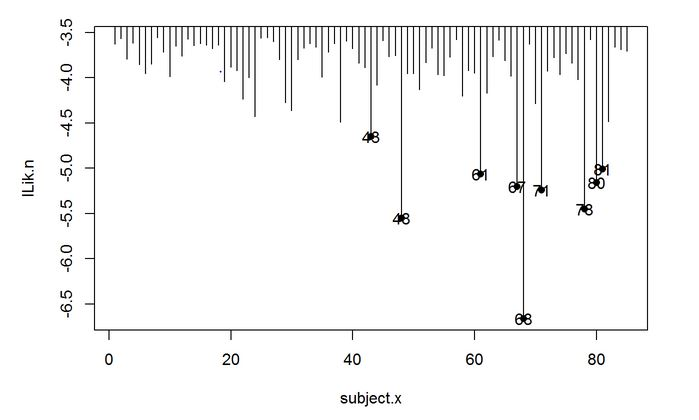
\includegraphics[width=0.7\linewidth]{images/LogLik-JS-Roy}
	\caption{}
	\label{fig:LogLik-JS-Roy}
\end{figure}

















\end{document}


